\documentclass[slidestop,compress,mathserif]{beamer}
\usepackage{fontspec,xunicode,xltxtra,beamerthemesplit}
\usepackage{graphicx}
\usepackage{color}
\usepackage{xcolor}
\usepackage{multicol}
\usepackage{animate}

\graphicspath{{figures/}}

%以下是各种演示主题,定义幻灯片中的所有细节
%\usetheme{default}
%\usetheme{Berlin}%这个主题比较好
%\usetheme{Pittsburgh}
%\usetheme{Rochester}
\usetheme{Berkeley}%这种演示主题比较好
%\usetheme{Goettingen}
%\usetheme{Hannover}
%\usetheme{Marburg}
%\usetheme{PaloAlto}%这种演示主题比较好
%\usetheme{Antibes}
%\usetheme{Darmstadt}
%\usetheme{JuanLesPins}
%\usetheme{Montpellier}
%\usetheme{Singapore}
%\usetheme{Boadilla}
%\usetheme{Madrid}
%\usetheme{AnnArbor}
%\usetheme{CambridgeUS}
%\usetheme{Copenhagen}
%\usetheme{Warsaw}

%以下是各种外部主题,确定幻灯的显示式样
%\useoutertheme{infolines}
%\useoutertheme{miniframes}
%\useoutertheme[height=0.1\textwidth,width=0.15\textwidth,hideothersubsections]{sidebar}
%\useoutertheme{smoothbars}
%\useoutertheme{split}
%\useoutertheme{shadow}
%\useoutertheme{tree}
%\useoutertheme{smoothtree}
%\useoutertheme[height=0.5\textwidth]{sidebar}

%以下是各种内部主题
%\useinnertheme{default}
%\useinnertheme{circles}
%\useinnertheme{rectangles}
\useinnertheme[shadow]{rounded}

%以下是各种颜色主题
%\usecolortheme{default}
%\usecolortheme{albatross}
%\usecolortheme{beaver}
%\usecolortheme{beetle}
%\usecolortheme{crane}
%\usecolortheme{dolphin}
%\usecolortheme{dove}
%\usecolortheme{fly}
%\usecolortheme{lily}
%\usecolortheme{orchid}
%\usecolortheme{rose}
%\usecolortheme{seagull}
\usecolortheme{seahorse}
%\usecolortheme{sidebartab}
%\usecolortheme{structure}
%\usecolortheme{whale}
%\usecolortheme{wolverine}

%以下是各种字体主题
%\usefonttheme{default}
%\usefonttheme[onlymath]{serif}
%\usefonttheme{structurebold}
%\usefonttheme{structureitalicserif}
%\usefonttheme{structuresmallcapsserif}

\setsansfont[Mapping=tex-text, BoldFont={Microsoft YaHei Bold}]{Microsoft YaHei}


% 中文环境自动换行
\XeTeXlinebreaklocale "zh"  % 表示用中文的断行
\XeTeXlinebreakskip = 0pt plus 1pt % 多一点调整的空间

% 中文环境修正导航栏
\makeatletter
\setbeamertemplate{blocks}[rounded][shadow=true] 
\def\beamer@linkspace#1{
  \begin{pgfpicture}{0pt}{-1.5pt}{#1}{5.5pt}
    \pgfsetfillopacity{0}
    \pgftext[x=0pt,y=-1.5pt]{.}
    \pgftext[x=#1,y=5.5pt]{.}
  \end{pgfpicture}}
\makeatother

% 超链接高亮显示
\hypersetup{CJKbookmarks=true,
colorlinks=true,
citecolor=blue,
linkcolor=blue,
urlcolor=blue,
bookmarksopen=true,
breaklinks=true
}


% 幻灯片切换方式
%\transblindshorizontal 	% 水平百叶窗
%\transblindsvertical 		% 垂直百叶窗
%\transboxin				% 盒状收缩
%\transboxout				% 盒状展开
%\transdissolve				% 溶解
%\transglitter
%\transsplithorizontalin	% 上下向中央收缩
%\transsplitverticalin		% 垂直向中央收缩
%\transsplithorizontalout	% 上下向中央展开
%\transsplitverticalout		% 垂直向中央展开
%\transwipe					% 从下抽出


\title{2002年图灵奖~\\~公钥密码学~\\~RSA加密算法}
\author{刘正~~徐小奇}
\date{\today}
%\institute{同济大学电信学院}

\logo{\color{blue!50}\scalebox{2}{{
\includegraphics[height=0.8cm]{logo.jpg}\vspace{220pt}}}}

% 设定frametitle居中
\makeatletter 
\long\def\beamer@@frametitle[#1]#2{% 
  \beamer@ifempty{#2}{}{% 
    \gdef\insertframetitle{\centering{#2\ifnum\beamer@autobreakcount>0\relax{}\space\usebeamertemplate*{frametitle continuation}\fi}}% 
  \gdef\beamer@frametitle{#2}% 
  \gdef\beamer@shortframetitle{#1}% 
}% 
} 
\makeatother


\begin{document}

\frame{\titlepage}

\section{RSA加密算法}

\begin{frame}
  \frametitle{加密的历史}
  
  \begin{block}<+->{1976年以前,所有的加密方法都是同一种模式:}
    \begin{itemize}[<+->]
        \item 甲方选择某一种加密规则,对信息进行加密;
        \item 乙方使用同一种规则,对信息进行解密。
    \end{itemize}
  \end{block}

\end{frame}

\begin{frame}
  \frametitle{加密的历史}
  
  \begin{block}{1976年以前,所有的加密方法都是同一种模式:}
    \begin{itemize}
        \item 甲方选择某一种加密规则,对信息进行加密;
        \item 乙方使用同一种规则,对信息进行解密。
    \end{itemize}
  \end{block}
  ~\\[0.6cm]

~ ~ ~ ~由于加密和解密使用同样规则(简称"密钥"),这被称为"对称加密算法"(Symmetric-key algorithm)。

~ ~ ~ ~这种加密模式有一个最大弱点:甲方必须把加密规则告诉乙方,否则无法解密。保存和传递密钥,就成了最头疼的问题。
\end{frame}

\subsection{\hfill 凯撒密码}
\begin{frame}
  \frametitle{凯撒密码}
  字母之间的替换---它的几个变种:换字式密码(破解的方法可以使用字符频数分析法)、转置式密码、多表替换密码(先分组后凯撒加密)
  \begin{figure}
    \centering
    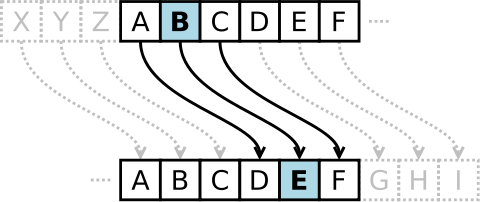
\includegraphics[width=5cm]{Caesar3.png}
  \end{figure}
\end{frame}

%\begin{frame}
%  \frametitle{凯撒密码}
%  \begin{itemize}[<+->]
%    \item{明文字母表:}ABCDEFGHIJKLMNOPQRSTUVWXYZ
%    \item{密文字母表:}DEFGHIJKLMNOPQRSTUVWXYZABC
%    \item{明文:}THE QUICK BROWN FOX JUMPS OVER THE LAZY DOG
%    \item{密文:}WKH TXLFN EURZQ IRA MXPSV RYHU WKH ODCB GRJ
%    \end{itemize}
%
%\end{frame}
%\begin{frame}
%  \frametitle{凯撒密码}
%  \begin{itemize}
%    \item{明文字母表:}ABCDEFGHIJKLMNOPQRSTUVWXYZ
%    \item{密文字母表:}DEFGHIJKLMNOPQRSTUVWXYZABC
%    \item{明文:}THE QUICK BROWN FOX JUMPS OVER THE LAZY DOG
%    \item{密文:}WKH TXLFN EURZQ IRA MXPSV RYHU WKH ODCB GRJ
%    \end{itemize}
%  恺撒密码的加密、解密方法还能够通过同余的数学方法进行计算。首先将字母用数字代替,A=0,B=1,\ldots,Z=25。此时偏移量为n的加密方法即为:
%
%  \begin{equation}
%    E_n=(x+n) ~mod~ 26
%  \end{equation}
%  解密就是:
%  \begin{equation}
%    D_n=(x-n) ~mod~ 26
%  \end{equation}
%
%\end{frame}


\subsection{\hfill 栅栏密码}
\begin{frame}
  \frametitle{栅栏密码}
加密的明文分成N个一组,然后把每组的第1个字连起来,形成一段无规律的话
\end{frame}

\subsection{\hfill 维基尼亚密码}


\subsection{\hfill 栅栏密码}
\begin{frame}
  \frametitle{栅栏密码}
加密的明文分成N个一组,然后把每组的第1个字连起来,形成一段无规律的话
\end{frame}

\subsection{\hfill 维基尼亚密码}
\begin{frame}
  \frametitle{维基尼亚密码}
引入密钥 对抗字频统计既同一个密文字符对应该的明文不一定是相同的)
\end{frame}

\begin{frame}
  \frametitle{RSA加密算法}
~ ~ ~ ~ RSA加密算法是一种非对称加密算法。在公开密钥加密和电子商业中RSA被广泛使用。

~ ~ ~ ~ RSA是1977年由罗纳德·李维斯特(Ron Rivest)、阿迪·萨莫尔(Adi Shamir)和伦纳德·阿德曼(Leonard Adleman)一起提出的。当时他们三人都在麻省理工学院工作。RSA就是他们三人姓氏开头字母拼在一起组成的。

~ ~ ~ ~ 1973年,在英国政府通讯总部工作的数学家克利福德·柯克斯(Clifford Cocks)在一个内部文件中提出了一个相同的算法,但他的发现被列入机密,一直到1997年才被发表。

\end{frame}

\section{获奖者生平}

\begin{frame}
  \frametitle{获奖啦}

\end{frame}


\subsection{\hfill Cocks}
\begin{frame}
  \frametitle{Clifford Cocks}
  \begin{multicols}{2}
    \begin{figure}
      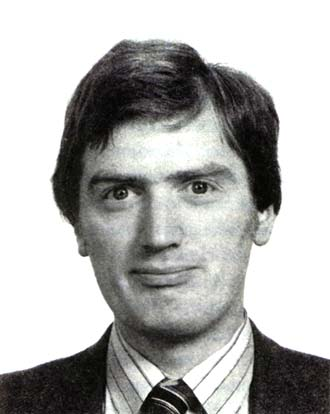
\includegraphics[width=3cm]{Cocks.jpg}
    \end{figure}
    Clifford Christopher Cocks出生于1950年12月28日,是英国数学家,密码学家,任职于英国国家通讯总部(GCHQ).
    
    He invented the widely used encryption algorithm now commonly known as RSA, about three years before it was independently developed by Rivest, Shamir, and Adleman at MIT. He has not been generally recognised for this achievement because his work was classified information, and therefore not released to the public at the time.

    
  \end{multicols}
  
\end{frame}

\subsection{\hfill Rivest}
\begin{frame}
  \frametitle{Ronald L. Rivest}
  \begin{multicols}{2}
    \begin{figure}
      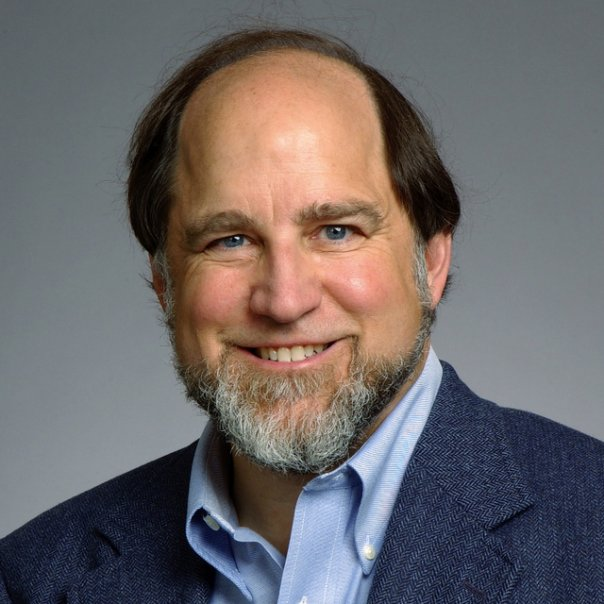
\includegraphics[width=3cm]{rivest_photo.jpg}
    \end{figure}
    
  \end{multicols}
  
\end{frame}

\subsection{\hfill Shamir}
\begin{frame}
  \frametitle{Adi Shamir}
  \begin{multicols}{2}
    \begin{figure}
      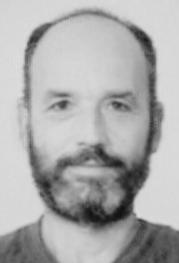
\includegraphics[width=3cm]{Shamir.jpg}
    \end{figure}
    
  \end{multicols}
  
\end{frame}

\subsection{\hfill Adleman}
\begin{frame}
  \frametitle{Leonard M. Adleman}
  \begin{multicols}{2}
    \begin{figure}
      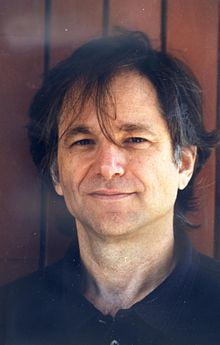
\includegraphics[width=3cm]{Adleman.jpg}
    \end{figure}
    
  \end{multicols}

\end{frame}





\section{八卦环节}









\begin{frame}
\frametitle{我是中文} 
%\framesubtitle{\centerline{subtext}} 
\animate<3-6>% 自动逐步显示
\begin{itemize}[<+->]
\item one
\item two
\item three
\item four
\item five
\item six
\end{itemize}

刘正 徐小奇 e
\end{frame}


















\end{document}
